\chapter{Results}\label{chap:results}
%\minitoc

\section{Chi2}

In this section we present a relevant test case to check the consistency of our
approach. We have selected a clean Si(001) surface with a $2\times 1$ surface
reconstruction. The slab for such a surface could be chosen to be
centrosymmetric by creating the front and back surfaces with the same $2\times
1$ reconstruction. However, we choose to terminate one of the surfaces with
hydrogen producing an ideal terminated bulk Si surface. The H atoms simply
saturate the dangling bonds of the bulk-like Si atoms at the surface, as seen in
Fig.~\ref{si2x1}. We take the $z$ coordinate pointing out of the surface and the
$x$ coordinate along the crystallographic [011] direction is parallel to the
dimmers.
\begin{figure}
\centering 
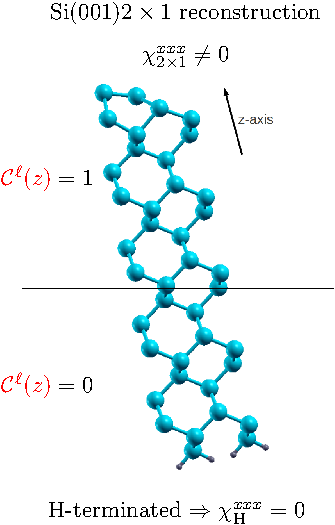
\includegraphics[scale=.8]{figures/03-results/chi2/fig2}
\caption{(color on line) The slab shows a 
clean Si(001)$2\times 1$ front surface with an ideal terminated Si bulk back
surface. The dangling bonds are H (small balls) saturated. This image depicts 12
Si atomic layers with one H atomic layer.
\label{si2x1}} 
\end{figure} 
The idea behind this slab configuration is that the cristalline symmetry of the
H terminated surface imposes that $\chi_{\mathrm{H}}^{xxx}=0$. The $2\times 1$
surface has no such restrictions, so $\chi_{2\times 1}^{xxx}\ne 0$. This is due
to the fact that along the $y$ direction there is a mirror plane for the
H-saturated surface, whereas for the $2\times 1$ surface this mirror is lost as
the dimers are asymmetric along $x$. Thus, calculating $\chi^{xxx}$ for the
full-slab, or the half-slab containing the $2\times 1$ surface\cite{note1}
should yield the same result since the contribution from the H saturated surface
is zero regardless. We must check that the following relationship is satisfied
for this particular slab
\begin{equation*}
\chi_{\mathrm{half-slab}}^{xxx}(-2\omega;\omega,\omega) 
=
\chi_{\mathrm{full-slab}}^{xxx}(-2\omega;\omega,\omega) 
,
\end{equation*}
where $\chi_{\mathrm{half-slab}}^{xxx}(-2\omega;\omega,\omega)$ is calculated
using ${\mathbf{\cal C}}(z)=1$ from the upper half containing the $2\times 1$
surface reconstruction, as seen in Fig.~\ref{si2x1}, and
$\chi_{\mathrm{full-slab}}^{xxx}(-2\omega;\omega,\omega)$ is calculated using
${\mathbf{\cal C}}(z)=1$ through the full slab. We show the results for this
comparison in the remainder of this section. Also, we checked that for the
dihydride surface $\chi_{\mathrm{half-slab}}^{xxx}(-2\omega;\omega,\omega)=0$.

The self-consistent ground state and the Kohn-Sham states were calculated in the
DFT-LDA framework using the plane-wave ABINIT code.\cite{abinit} We used
Troullier-Martins pseudopotentials\cite{troullierPRB91} that are fully separable
nonlocal pseudopotentials in the Kleinman-Bylander form.\cite{kleinmanPRL82} The
contribution of $\mathbf{v}^\mathrm{nl}$ and $\boldsymbol{\mathcal{\cal
V}}^\mathrm{nl}$ to Eq.~\eqref{chis} is carried out using the DP
code.\cite{olevanoDP} The surfaces have been studied with the experimental
lattice constant of 5.43 \AA. Structural optimizations were performed with the
ABINIT code.\cite{abinit} The geometry optimization has been carried out in
slabs of 12 atomic layers where the central four layers where fixed at the bulk
positions. The structures were relaxed until the Cartesian force components were
less than 5 meV/\AA. The geometry optimization for the clean surface gives a
dimer buckling of 0.721 \AA, and a dimer length of 2.301 \AA. For the
Si(001)$1\times 1$:2H dihydride surface, we have obtained a Si-H bond distance
of 1.48 \AA. This results are in good agreement with previous theoretical
studies.\cite{caramellaPRB09,mendozaPRB06} The vacuum size is equivalent to one
quarter the size of the slab, avoiding the effects produced by possible
wave-function tunneling from the contiguous surfaces of the full crystal formed
by the repeated super-cell scheme.\cite{mendozaPRB06}

Spin-orbit, local field, and electron-hole attraction\cite{beyond} effects on
the SHG process are all neglected. Although these are important factors in the
optical response of a semiconductor, their efficient calculation is still
theoretically and numerically challenging and under debate. This merits further
study but is beyond the scope of this paper. For a given slab size, we find the
converged spectra to obtain the relevant parameters. The most important of these
are: an energy cut-off of 10 Ha for the 16, 24, and 32 layered slabs and 13 Ha
for the 40 layer slab, an equal number of conduction and valence bands, and a
set of 244 $\mathbf{k}$-points. The $\mathbf{k}$-points are used for the linear
analytic tetrahedron method for evaluating the 3D Brillouin Zone (BZ) integrals
where special care was taken to examine the double resonances of
Eq.~\eqref{chis}. \cite{nastosPRB05} Note that the Brillouin zone for the slab
geometry collapses to a 2D-zone, with only one $\mathbf{k}$-point along the
$z$-axis. All spectra were calculated with a Gaussian smearing of 0.15 eV.
\begin{figure}
\centering 
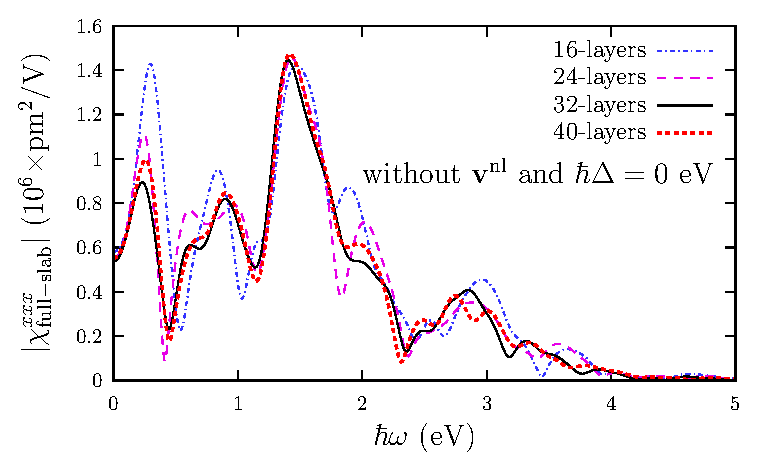
\includegraphics[scale=.8]{figures/03-results/chi2/fig3}
\caption{(color on line) 
$|\chi_{\mathrm{half-slab}}^{xxx}|$ vs $\hbar\omega$ for the slab with 16, 24,
32, and 40 atomic Si layers. The front surface is in a clean $2\times 1$
reconstruction and the back surface is an ideal terminated bulk H-saturated
dangling bonds (see Fig.~\ref{si2x1}).
\label{fig1}} 
\end{figure}
\begin{figure}
\centering 
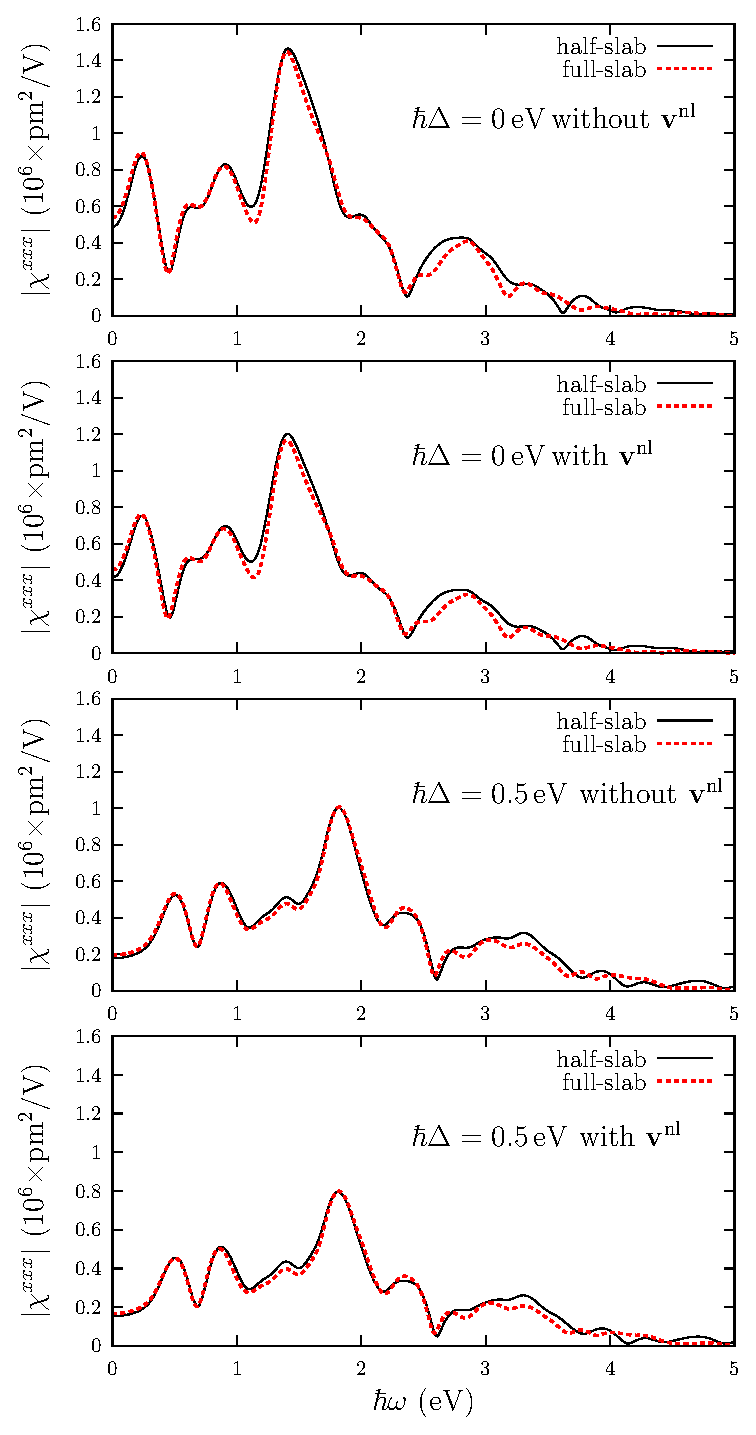
\includegraphics[scale=.8]{figures/03-results/chi2/fig4}
\caption{(color on line) 
$\chi^{xxx}_{\mathrm{half-slab}}$ and $\chi^{xxx}_{\mathrm{full-slab}}$ vs
$\hbar\omega$ for a slab with 32 atomic Si layers plus one H layer.
\label{fig2}} 
\end{figure}

We must evaluate $T^{\mathrm{a}\mathrm{b}}_{nm}=(i/\hbar)[r^\mathrm{b},v^{\mathrm{nl},\mathrm{a}}]_{nm}$ in order to obtain Eqs.~\eqref{tau.1} and
\eqref{tau.1n} that are required for Eq.~\eqref{chis}. Computing second-order
derivatives is required thus making the numerical procedure very time consuming.
This adds significantly to the already lengthy time needed for the calculation
of the $\mathbf{v}^\mathrm{nl}$ contribution that is proportional only to the
first order derivatives. Memory requirements are also increased for both
$\mathbf{v}^\mathrm{nl}$ and $[\mathbf{r},\mathbf{v}^\mathrm{nl}]$. However, the
contribution from $[\mathbf{r},\mathbf{v}^\mathrm{nl}]$ is very
small\cite{valerie} and therefore we neglect it in this work.


\subsection{Full-slab results}\label{fsresults}

In Fig.~\ref{fig1} we show $|\chi_{\mathrm{full-slab}}^{xxx}|$ for the slab with
16, 24, 32, and 40 Si atomic layers, without the contribution of
$\mathbf{v}^{\mathrm{nl}}$ and with no scissors correction. Since the clean
Si(001) surface is $2\times 1$, there are two atoms per atomic layer, thus the
total number of atoms per slab is twice the number of atomic layers of the slab.
In making the slabs larger, we add steps of 8 layers of bulk-like atomic
positions. We note that the response differs substantially for 16 and 24 layers
but is quite similar for 32 and 40 layers. As explained above, the calculation
of the $\mathbf{v}^\mathrm{nl}$ contribution is computationally expensive. A
good compromise between the accuracy in the convergence of
$\chi^{xxx}_{\mathrm{full-slab}}$ as a function of the number of layers in the
slab, and the computational expense is to consider the slab with 32 Si atomic
layers as an accurate representation of our system.


\subsection{Half-slab vs. full-slab}

In Fig.~\ref{fig2} we compare $\chi^{xxx}_{\mathrm{half-slab}}$ vs.
$\chi^{xxx}_{\mathrm{full-slab}}$ for the four different possibilities between
including or not including the effects of $\mathbf{v}^\mathrm{nl}$ or the
scissors correction $\hbar\Delta$. For these results we chose $\hbar\Delta=0.5$
eV, that is the GW gap reported in Refs. \cite{rohlfingPRB95,garciaCPC01}.
This is justified by the fact that the surface states of the clean Si(001)
surface are rigidly shifted and maintain their dispersion relation with respect
to LDA according to the GW calculations of Ref. \cite{rohlfingPRB95}. We
see that for all four instances the difference between responses is quite small.
Indeed, when the value $|\chi^{xxx}|$ is large the difference between the two is
very small; when the value is small the difference increases only slightly, but
the spectra is so close to zero that it is negligible. These differences would
decrease as the number of atomic layers increases. We remark that 32 layers in
the slab is more than enough to confirm that the extraction of the surface
second-harmonic susceptibility from the $2\times 1$ surface is readily possible
using the formalism contained in Eq.~\eqref{chis}. We have confirmed that for
the dihydride surface $|\chi^{xxx}_{\mathrm{half-slab}}|\approx 0$ (not shown).
This confirms the validity of our theory and is the main result of this article;
through the proposed layer formalism we can calculate the surface SH
$\chi^{\mathrm{a}\mathrm{b}\mathrm{c}}(-2\omega;\omega,\omega)$ including the
contribution of the nonlocal part of the pseudopotentials and the part of the
many-body effects through the scissors correction. Our scheme should work for
any slab.

\subsection{\texorpdfstring{Results for $\chi^{xxx}_{2\times 1}(-2\omega;\omega,\omega)$}
{Results for Xxxx(2x1)(-2w;w,w)}}

We proceed to explain some of the features seen in $|\chi^{xxx}_{2\times 1}|$
that, as explained above, are obtained by calculating
$|\chi^{xxx}_{\mathrm{half-slab}}|$. First, from Fig.~\ref{fig2} we note a
series of resonances that derive from 1$\omega$ and 2$\omega$ terms in
Eq.~\eqref{chis}. Notice that the 2$\omega$ resonances start below $E_g/2$ where
$E_g$ is the band gap (0.53 eV  for LDA and 1.03 eV if the scissor is used with
$\hbar\Delta=0.5$ eV). These resonances come from the electronic states of the
$2\times 1$ surface, that lie inside the bulk band gap of Si and are the well
known electronic surface states.\cite{rohlfingPRB95} In Fig.~\ref{fig3} we see
that the effect of $\mathbf{v}^\mathrm{nl}$ reduces the value of
$|\chi^{xxx}_{2\times 1}|$ by 15-20\% showing the importance of this
contribution for a correct calculation of SSHG, in agreement with the analysis
for bulk semiconductors.\cite{luppiPRB08} However, the inclusion of
$\mathbf{v}^\mathrm{nl}$ does not changes the spectral shape of
$|\chi^{xxx}_{2\times 1}|$; this also can be confirmed from the cases of zero
scissors correction from Fig.~\ref{fig2}.
\begin{figure}
\centering 
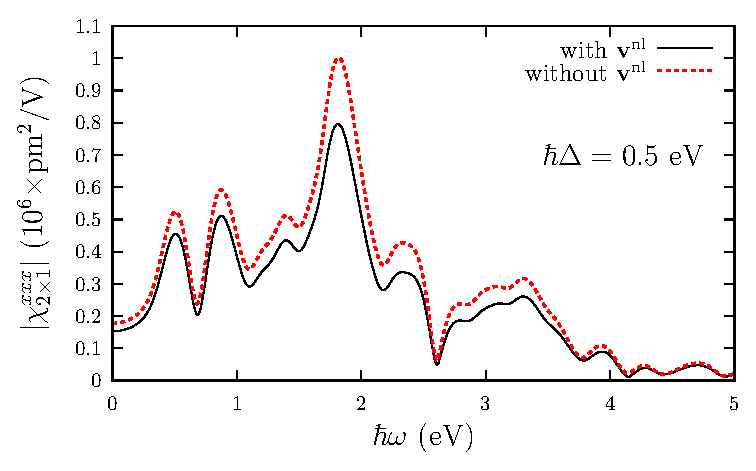
\includegraphics[scale=.8]{figures/03-results/chi2/fig5}
\caption{(color on line) 
$\chi^{xxx}_{2\times 1}$ vs $\hbar\omega$ for a slab with 32 atomic Si layers
plus one H layer, with and without the contribution from
$\mathbf{v}^\mathrm{nl}$.
\label{fig3}} 
\end{figure}

To see the effect of the scissors correction, we take two different finite
values for $\hbar\Delta$. The first one with a value of $\hbar\Delta=0.5$ eV,
used in the above results, is the ``average'' GW gap taken from
Ref. \cite{rohlfingPRB95} that is in agreement with
Ref. \cite{garciaCPC01}. The second one with a value of $\hbar\Delta=0.63$
eV is the ``average'' gap taken from Ref. \cite{asahiPRB00}, where more
$\mathbf{k}$-points in the Brillouin zone were used to calculate its GW value.
From Fig.~\ref{fig4} we note that the scissors correction shifts the spectra
from its LDA value to higher energies as expected. However, contrary to the case
of linear optics\cite{cabellosPRB09} the shift introduced by the scissors
correction is not rigid, as pointed out in Ref. \cite{nastosPRB05}. This
is because the second-harmonic optical response mixes $1\omega$ and $2\omega$
transitions (see Eq.~\eqref{chis}), and accounts for the non-rigid shift. The
reduction of the spectral strength is in agreement with previous calculations
for bulk systems.\cite{nastosPRB05, luppiPRB10, leitsmannPRB05} When we compare
$|\chi^{xxx}_{2\times 1}|$ for the two finite values of $\hbar\Delta$, we see
that the first two peaks are almost rigidly shifted with a small difference in
height while the rest of the peaks are modified substantially. This behavior
comes from the fact that the first two peaks are almost exclusively related to
the 2$\omega$ resonances of Eq.~\eqref{chis}. The other peaks are a combination
of 1$\omega$ and 2$\omega$ resonances and yield a more varied spectrum. We
mention that for large gap materials, the 1$\omega$ and 2$\omega$ would be
splited showing a small interference effect, but still the 2$\omega$ would
strongly depend on the surface states. This way we see that small changes in the
value of the scissors shift can in general affect the SSH susceptibility
spectrum quite dramatically. In Ref. \cite{adolphPRB00}, the authors
already remarked that nonlinear optical response of bulk materials is more
influenced by the electronic structure of the material than the linear case. In
the case of semiconducting surfaces the problem is even more intricate due to
the presence of electronic surface states. The high sensitivity of SSHG to the
energy position  of surface states, as seen in Fig.~\ref{fig4}, makes SSHG a
good benchmark spectroscopical tool for testing the validity of the inclusion of
many-body effects, and in particular the quasi-particle correction to the
electronic states.
\begin{figure}
\centering 
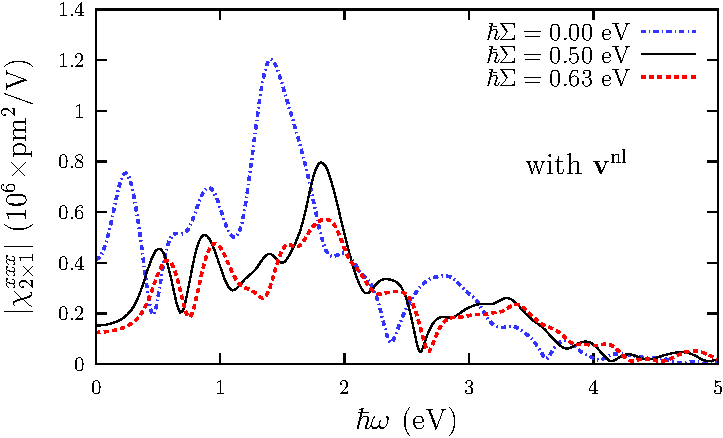
\includegraphics[scale=.8]{figures/03-results/chi2/fig6}
\caption{(color on line) 
$\chi^{xxx}_{2\times 1}$ vs $\hbar\omega$ for a slab with 32 atomic Si layers
plus one H layer, for two different values of the scissors correction
$\hbar\Delta$.
\label{fig4}} 
\end{figure}

Although local fields are neglected they should, in principle, be small parallel
to the interface as the electric field is continuous. So, we would expect that
the $xxx$ component of $\boldsymbol{\chi}(-2\omega;\omega,\omega)$ would have a
small influence from the local fields. Also, the excitonic effects ought to be
explored, but their efficient calculation is theoretically and numerically
challenging\cite{beyond}   and beyond the scope of this article. Unfortunately
the experimental measurement of the $xxx$ component of
$\boldsymbol{\chi}(-2\omega;\omega,\omega)$ is not possible as the SH radiated
intensity would be proportional not only to this component but also to the other
components of $\boldsymbol{\chi}(-2\omega;\omega,\omega)$. However, in a
forthcoming publication we will present a study of SSHG from several Si surfaces
with comparison to experimental results.


\section{SHG Yield}

\section{Method}\label{sec:method}

We constructed the Si(111)(1$\times$1):H surface with the experimental lattice
constant of 5.43 \AA, and then performed structural optimizations with the
ABINIT\cite{gonzeCPS09, abinit} code. The structures were relaxed until the
Cartesian force components were less than 5 meV/\AA, yielding a final Si-H bond
distance of 1.50 \AA. The energy cutoff used was 20 Ha, and we used
Troullier-Martin LDA pseudopotentials.\cite{troullierPRB91} The resulting atomic
positions are in good agreement with previous theoretical studies,
\cite{kaxirasPRB88, jonaPRB95, alfonsoPRB96, cargnoniJOCP00, mejiaPRB02} as well
as the experimental value for the Si-H distance.\cite{weastCRC88}

We also evaluated the number of layers required for convergence and settled on a
slab with 48 atomic Si planes. The geometric optimizations mentioned above are
therefore carried out on slabs of 48 atomic layers without fixing any atoms to
the bulk positions. All of the calculations involve
$\epsilon^{\mathrm{ab}}_{\mathrm{half-slab}}$ and
$\chi^{\mathrm{abc}}_{\mathrm{half-slab}}$, which are calculated with
${\mathbf{\mathcal{C}}}(z)=1$ for the upper half of our slab. This encompasses
24 layers of Si and the single layer of H that terminates the top surface. The
vacuum size is equivalent to one quarter the size of the slab, avoiding the
effects produced by possible wave-function tunneling from the contiguous
surfaces of the full crystal formed by the repeated super-cell
scheme.\cite{mendozaPRB06}

The electronic wave-functions, $\psi_{n\mathbf{k}}(\mathbf{r})$, were also
calculated with the ABINIT code using a planewave basis set with an energy
cutoff of 15 Hartrees. $\chi^{\mathrm{abc}}(-2\omega;\omega,\omega)$ was
properly converged with 576 \textbf{k} points in the irreducible Brillouin zone,
which are equivalent to 1250 \textbf{k} points if we disregard symmetry
relations. The contribution of $\boldsymbol{\mathcal{\cal V}}^\mathrm{nl}$ in
Eq.~\eqref{eq:chis} was carried out using the DP\cite{olevanoDP} code with a
basis set of 3000 planewaves. Convergence for the number of bands was achieved
at 200, which includes 97 occupied bands and 103 unoccupied bands.

All spectra were produced using a scissors value of 0.7\,eV in the
$\chi^{\mathrm{abc}}(-2\omega;\omega,\omega)$ and
$\boldsymbol{\epsilon}_{\ell}(\omega)$ calculations. This value was obtained
from Ref. \cite{liPRB10}, in which the authors carry out a
$\mathrm{G}_{0}\mathrm{W}_{0}$ calculation on this surface for increasing
numbers of layers. They calculated the LDA and $\mathrm{G}_{0}\mathrm{W}_{0}$
band gaps, and found that the difference between the two tends towards
$\sim0.7$\,eV as more layers are added, culminating in a value of 0.68\,eV for
bulk Si. This calculation is completely \emph{ab-initio}, so we choose 0.7\,eV
as a very reasonable value for the scissors correction.

Our method of calculation is as follows. We first calculated
$\varepsilon_{b}(\omega)$, $\varepsilon_{\ell}(\omega)$, and then
$\chi^{\mathrm{abc}}(-2\omega;\omega,\omega)$ from Eq. \eqref{eq:chis}. We used
these for the Fresnel factors and in Eqs. \eqref{eq:rpP}, \eqref{eq:rpS}, and
\eqref{eq:rsP}, and finally, those into Eq. \eqref{eq:r19} to obtain the
theoretical SHG yield for different polarizations that can then be compared with
the experimental data.


\section{Results}\label{sec:results}

In this section, we present our theoretical results compared with the
appropriate experimental data. For full details on these experiments, see Refs.
\cite{hoferAPA96, mitchellSS01, mejiaPRB02, bergfeldPRL04}. This analysis
provides information on the physics behind the SHG yield and how it is affected
by a variety of factors.


\subsection{Calculating
\texorpdfstring{$\boldsymbol{\chi}(-2\omega;\omega,\omega)$}{X(-2w;w,w)} using
relaxed atomic positions}\label{sec:relaxed}

The pioneering work presented in Ref. \cite{mejiaPRB02} showed the effect
of artificially moving the atomic position on the resulting SSHG spectra. In
this section, we address the more practical and relevant case of atomic
relaxation. More precisely, we compare the fully relaxed structure described in
Sec. \ref{sec:method} with an unrelaxed structure where all the Si atoms are at
the ideal bulk positions. Note that in both cases, the Si-H bond distance is the
same 1.5\,\AA.

We compare the calculated $\chi^{xxx}(-2\omega;\omega,\omega)$ with experimental
data for this surface taken from Ref. \cite{hoferAPA96}. This data
provides an excellent point of comparison as it was presented in absolute units
and was measured at a very low temperature of 80 K. We used both relaxed (as
detailed in Sec. \ref{sec:method}) and unrelaxed atomic positions to calculate
the nonlinear susceptibility tensor. The calculation with the unrelaxed
coordinates was done with the same parameters mentioned above.

We can see from Fig. \ref{fig:Xxxx} that the relaxed coordinates have an
improved peak position that is very slightly blueshifted with respect to the
experimental peak near 1.7\,eV. In contrast, the unrelaxed coordinates have a
peak that is redshifted close to 0.05\,eV from experiment. There is also a
feature between 1.5\,eV and 1.6\,eV that appears in the relaxed spectrum that
coincides partially with the experimental data. It is important to note that
this data was taken at low temperature (80 K); this further favors the
comparison, as the theory neglects the effects of temperature. We can also see
from Ref. \cite{hoferAPA96} that the peaks in the spectrum redshift as
the temperature increases. Intensity for both the relaxed and unrelaxed curves
are roughly half the intensity of the experimental spectrum. We have converted
the units of the experimental data from CGS to MKS units for easier comparison.

\begin{figure}[t]
\centering
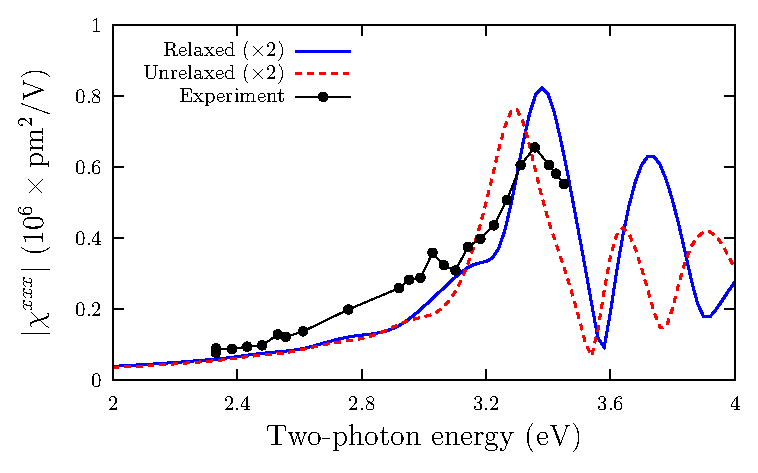
\includegraphics[width=0.48\textwidth]{figures/03-results/shgyield/fig2}
\caption{(Color online) Comparison of $\chi^{xxx}(-2\omega;\omega,\omega)$
calculated using relaxed and unrelaxed atomic positions, with the experimental
data presented in Ref. \cite{hoferAPA96}. Theoretical curves are broadened
with $\sigma=0.05\,\text{eV}$.\label{fig:Xxxx}}
\end{figure}

Therefore, the most accurate theoretical results are given by using relaxed
atomic positions for the calculation of
$\boldsymbol{\chi}(-2\omega;\omega,\omega)$. Although this process can be very
time consuming for large numbers of atoms, we consider it a crucial step. From a
numerical standpoint, this further demonstrates that SSHG is very sensitive to
the surface atomic positions. In particular, our results show that a correct
value of the Si-H bond length is not enough to obtain the most accurate SSHG
spectra, and that a full relaxation of the structure is required. Additionally,
experiments that are conducted under very low temperature conditions will also
yield improved similarity with theory.


\subsection{Calculated \texorpdfstring{$\mathcal{R}_{pS}$}{RpS} compared to
experiment}\label{sec:RpS}

All calculations presented from this point on were done using the relaxed atomic
positions described in previous sections. We now move on to the theoretical SHG
yield compared with experiment. We first compare the calculated
$\mathcal{R}_{pS}$ spectra with room temperature experimental data from Ref.
\cite{mejiaPRB02}. We adhere to the experimental setup by taking an angle
of incidence $\theta=65^{\circ}$ and an azimuthal angle of $\phi=30^\circ$ with
respect to the $x$-axis. This azimuthal angle maximizes $r_{pS}$, as shown in
Eq. \eqref{eq:rpS}. In Fig. \ref{fig:RpS}, we see that the three layer model
accurately reproduces the lineshape of the experimental spectrum which includes
the peaks corresponding to both the E$_{1}$ (3.4\,eV) and E$_{2}$ (4.3\,eV)
critical points of bulk silicon, and a smaller feature at around 3.8\,eV. The
calculated E$_{1}$ and E$_{2}$ peaks are redshifted by 0.1\,eV and 0.06\,eV,
respectively, compared with the experimental peaks. The intensity using this
model is very close to that measured in the experiment. 

\begin{figure}[b]
\centering
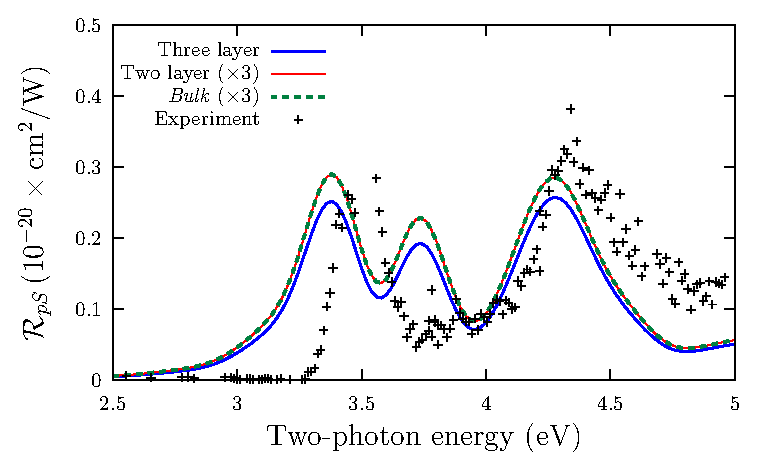
\includegraphics[width=0.48\textwidth]{figures/03-results/shgyield/fig3}
\caption{(Color online) Comparison between theoretical models (see Table
\ref{tab:models}) and experiment for $\mathcal{R}_{pS}$, for
$\theta=65^{\circ}$. We use a scissors value of $\hbar\Delta = 0.7\,\text{eV}$.
The $\chi^{\mathrm{abc}}(-2\omega;\omega,\omega)$ components are broadened with
$\sigma=0.05\,\text{eV}$, and then $\mathcal{R}_{pS}$ is broadened with
$\sigma=0.10\,\text{eV}$. Experimental data taken from Ref.
\cite{mejiaPRB02}.\label{fig:RpS}}
\end{figure}

The main issue to address here is the discrepancy between the intensity of the
E$_{1}$ peak. In the theoretical curves, the peaks differ only slightly in
overall intensity. Conversely, the experimental E$_{1}$ peak is significantly
smaller than the E$_{2}$ peak. This may be due to the effects of oxidation on
the surface. Ref. \cite{bergfeldPRL04} features similar data to those of
Ref. \cite{mejiaPRB02} but focuses on the effects of surface oxidation. We
can see that as time passes during the experiment, the surface becomes more
oxidized, and the E$_{1}$ peak diminishes substantially, as shown by the
experimental data taken 5 hours after initial H-termination. This may be enough
time to slightly reduce the E$_{1}$ peak intensity, as can be observed here.

In Fig. \ref{fig:mitchellRpS}, we compare the theoretical $\mathcal{R}_{pS}$
with experimental data from Ref. \cite{mitchellSS01}; this data, however,
only encompasses the E$_{1}$ peaks, and was obtained at room temperature. We
consider an angle of incidence $\theta=45^\circ$ and an azimuthal angle
$\phi=30^\circ$ to match these experimental conditions. As in the previous
comparison, the E$_{1}$ peak is slightly redshifted compared to experiment. The
intensity of the theoretical yield is smaller than the experimental yield for
all three models. The measurements presented in Ref. \cite{mitchellSS01}
were taken very shortly after the surface had been prepared, and the surface
itself was prepared with a high degree of quality and measured at room
temperature. Peak position compared to theory is slightly improved under these
conditions. As before, the three layer model is closer in intensity to the
experimental spectrum.

\begin{figure}[b]
\centering
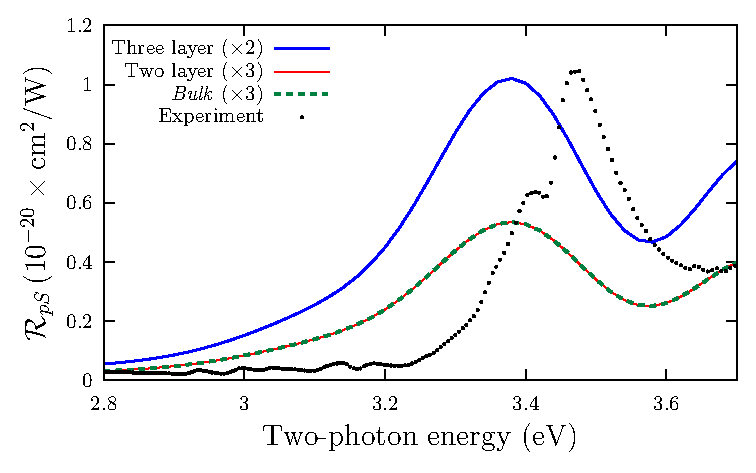
\includegraphics[width=0.48\textwidth]{figures/03-results/shgyield/fig4}
\caption{(Color online) Comparison between theoretical models (see Table
\ref{tab:models}) and experiment for $\mathcal{R}_{pS}$, for $\theta=45^\circ$.
We use a scissors value of $\hbar\Delta = 0.7\,\text{eV}$. The
$\chi^{\mathrm{abc}}(-2\omega;\omega,\omega)$ components are broadened with
$\sigma=0.05\,\text{eV}$, and then $\mathcal{R}_{pS}$ is broadened with
$\sigma=0.10\,\text{eV}$. Experimental data taken from Ref.
\cite{mitchellSS01}.\label{fig:mitchellRpS}}
\end{figure}

In both comparisons, the E$_{1}$ peak position is slightly redshifted. It is well
known that temperature causes shifting in the peak position of SHG
spectra.\cite{dadapPRB96} We showed in the previous section that our calculation
is closer to low temperature measurements. It is likely that low temperature
measurements for the SHG yield will lead to more closely matched results.

Both the two layer and bulk models are identical and roughly 3 times smaller
than the experiment. We can see from Eq. \eqref{eq:rpS} that $\mathcal{R}_{pS}$
only has $1\omega$ terms ($\varepsilon_{\ell}(\omega)$ and $k_{b}$). For both of
these models, the fundamental fields are evaluated in the bulk, which means that
the only change to Eq. \eqref{eq:rpS} is that $\varepsilon_{\ell}(\omega)
\rightarrow \varepsilon_{b}(\omega)$. Additionally, $\Gamma^{\ell}_{pS}$ also
remains identical between the two models and has no $2\omega$ terms in the
denominator. Therefore, $r_{pS}$ is identical between these two models.
Ultimately, the three layer model best reproduces both the lineshape and the
intensity of the experimental spectrum.

Per Eq. \eqref{eq:rpS}, the intensity of $\mathcal{R}_{pS}$ depends only on
$\chi_{\parallel\parallel\parallel}$, which is not affected by local field
effects.\cite{tancognedejean:tel-01235611} These effects are neglected in this
calculation, but $\mathcal{R}_{pS}$ maintains an accurate lineshape and provides
a good quantitative description of the experimental SHG yield. We note that both
the calculated and experimental spectra show two-photon resonances at the
energies corresponding to the critical point transitions of bulk Si. We also see
that the SHG yield drops rapidly to zero below E$_{1}$, which is consistent with
the absence of surface states due to the H saturation on the surface. This
observation holds true for all three polarization cases studied here.

Lastly, in Fig. \ref{fig:improvements} we provide an overview of the different
levels of approximation proposed in this article. All curves here were
calculated using the three layer model. The long dashed line depicts the effect
of excluding the contribution from the nonlocal part of the pseduopotentials.
This is consistent with the results reported in Ref. \cite{andersonPRB15},
where the exclusion of this term increases the intensity of the components of
$\boldsymbol{\chi}(-2\omega;\omega,\omega)$ by approximately 15\% to 20\%. We
also notice that the E$_{1}$ peak is larger than the E$_{2}$ peak, contrasting
with the experiment, where the E$_{1}$ peak is smaller than E$_{2}$. Lastly, the
thin solid line depicts the full calculation with a scissors value of
$\hbar\Delta = 0$. We notice that the spectrum is almost rigidly redshifted as
this H-saturated surface has no electronic surface states.\cite{andersonPRB15}
Thus, this demonstrates the importance of including the scissors correction to
accurately reproduce the experimental spectrum. In summary, the inclusion of the
contribution from the nonlocal part of the pseudopotentials and the scissors
operator on top of the three layer model gives a much better comparison with the
experimental data.

\begin{figure}[b]
\centering
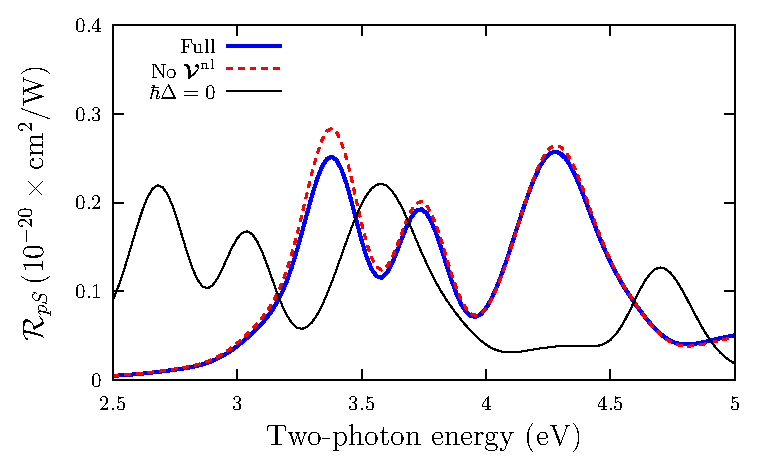
\includegraphics[width=0.48\textwidth]{figures/03-results/shgyield/fig5}
\caption{(Color online) Calculated results for $\mathcal{R}_{pS}$ for the
different levels of approximation proposed in this article. All curves were
calculated using the three layer model. We take $\theta=65^{\circ}$ for this
plot. See text for full details. The
$\chi^{\mathrm{abc}}(-2\omega;\omega,\omega)$ components are broadened with
$\sigma=0.05\,\text{eV}$, and then $\mathcal{R}_{pS}$ is broadened with
$\sigma=0.10\,\text{eV}$.
\label{fig:improvements}}
\end{figure}


\subsection{Calculated \texorpdfstring{$\mathcal{R}_{sP}$}{RsP} compared to
experiment}\label{sec:RsP}

Next, we analyze and compare the calculated $\mathcal{R}_{sP}$ spectra with
experimental data from Ref. \cite{mejiaPRB02}. We again adhere to the
experimental setup by taking an angle of incidence $\theta=65^{\circ}$ and an
azimuthal angle $\phi=30^\circ$. From Fig. \ref{fig:RsP}, we can immediately
appreciate that the overall intensity of $\mathcal{R}_{sP}$ is one order of
magnitude lower than $\mathcal{R}_{pS}$. The experimental data is far noisier
than in the other cases but we can still discern the E$_{1}$ and E$_{2}$ peaks.
As with our previous comparisons, the three layer model accurately matches both
the intensity and the lineshape of the experimental spectrum. It produces a
curve that is very close to the experimental intensity with good proportional
heights for the calculated E$_{1}$ and E$_{2}$ peaks. In contrast, the two layer
model is 100 times more intense than experiment and produces an enlarged E$_{2}$
peak. The bulk model is ten times smaller with a good lineshape.

The differences between the two layer and bulk models are not derived from Eq.
\eqref{eq:rsP}, as the $\varepsilon_{b}(2\omega)$ does not change and the second
term vanishes for this azimuthal angle of $\phi = 30$. However,
$\Gamma^{\ell}_{sP}$ does cause a significant change in the intensity as there
is an $\varepsilon_{\ell}(2\omega)$ term in the denominator. This will become
$\varepsilon_{v}(2\omega) = 1$ for the two layer model, and
$\varepsilon_{b}(2\omega)$ in the bulk model. This accounts for the significant
difference between the intensity of the two models, while the lineshape remains
mostly consistent.

At higher energies, the theoretical curve is blueshifted as compared to the
experiment. We consider that the likely explanation for this is the inclusion of
the scissor operator, which does not adequately correct the transitions
occurring at these higher energies. A full GW calculation would be well suited
for this task, but is beyond the scope of this paper.

\begin{figure}[t]
\centering
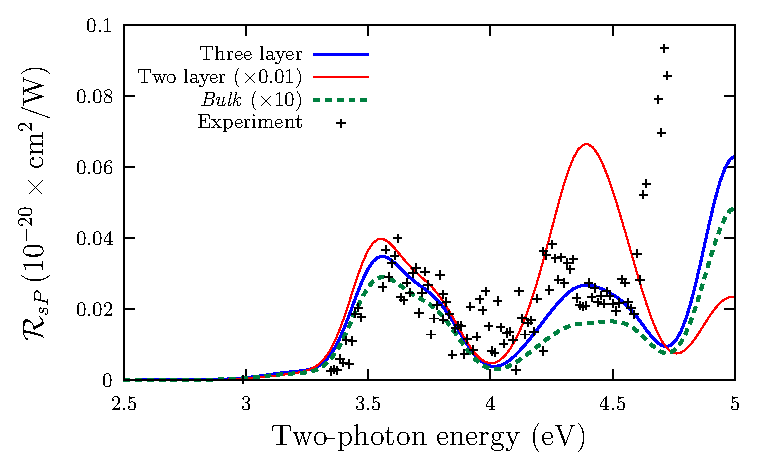
\includegraphics[width=0.48\textwidth]{figures/03-results/shgyield/fig6}
\caption{(Color online) Comparison between theoretical models (see Table
\ref{tab:models}) and experiment for $\mathcal{R}_{sP}$, for
$\theta=65^{\circ}$. We use a scissors value of $\hbar\Delta = 0.7\,\text{eV}$.
The $\chi^{\mathrm{abc}}(-2\omega;\omega,\omega)$ components are broadened with
$\sigma=0.05\,\text{eV}$, and then $\mathcal{R}_{sP}$ is broadened with
$\sigma=0.10\,\text{eV}$. Experimental data taken from Ref.
\cite{mejiaPRB02}.\label{fig:RsP}}
\end{figure}


\subsection{Calculated \texorpdfstring{$\mathcal{R}_{pP}$}{RpP} compared to
experiment}\label{sec:RpP}

We present $\mathcal{R}_{pP}$ compared to experimental data from Ref.
\cite{mejiaPRB02} in Fig. \ref{fig:RpP}. We note that peak position for
the three layer model is similar to experiment with the overall intensity being
only two times larger. The E$_{2}$ peak is blueshifted by around 0.3\,eV, and
the yield does not go to zero after 4.75\,eV. The two layer model has good
lineshape, but it is 40 times more intense than experiment. The calculated
E$_{2}$ peak is similar, but the E$_{1}$ peak lacks the sharpness present in the
experiment. The bulk model is very close to the lineshape of the three layer
model, but with four times less intensity. From Eq. \eqref{eq:rpP}, we see that
$\mathcal{R}_{pP}$ has several $2\omega$ terms that will change between models.
This will have a deep effect on the lineshape. Coupled to $\Gamma^{\ell}_{pP}$,
which also has $\varepsilon_{\ell}(2\omega)$ in the denominator, and we have a
significant difference in both lineshape and intensity between the two layer and
bulk models.

Reviewing Eq. \eqref{eq:rpP}, we see that $\mathcal{R}_{pP}$ is by far the most
involved calculation, since it includes all four nonzero components. In
particular, $\chi_{\perp\perp\perp}$ and $\chi_{\parallel\parallel\perp}$
include out-of-plane incoming fields. These are affected by local field effects
that can change both intensity and peak
position.\cite{tancognedejean:tel-01235611} Including these effects is
computationally very expensive and is beyond the scope of this paper. We
speculate that $\mathcal{R}_{pP}$ requires the proper inclusion of these effects
in order to accurately describe the experimental peaks.

\begin{figure}[b]
\centering
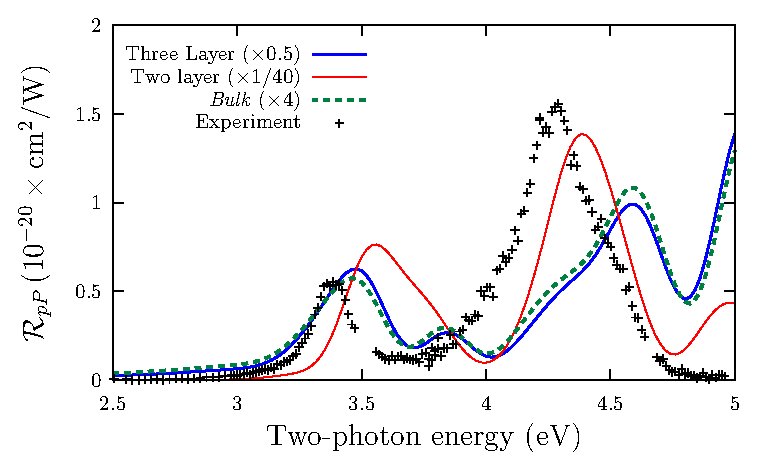
\includegraphics[width=0.48\textwidth]{figures/03-results/shgyield/fig7}
\caption{(Color online) Comparison between theoretical models (see Table
\ref{tab:models}) and experiment for $\mathcal{R}_{pP}$, for
$\theta=65^{\circ}$. We use a scissors value of $\hbar\Delta = 0.7\,\text{eV}$.
The $\chi^{\mathrm{abc}}(-2\omega;\omega,\omega)$ components are broadened with
$\sigma=0.05\,\text{eV}$, and then $\mathcal{R}_{pP}$ is broadened with
$\sigma=0.10\,\text{eV}$. Experimental data taken from Ref.
\cite{mejiaPRB02}.\label{fig:RpP}}
\end{figure}

Lastly, in Fig. \ref{fig:mitchellRpP} we compare to Ref.
\cite{mitchellSS01}. The three layer model is, as before, very close in
both peak position and intensity. Intensity is improved with the calculated
spectrum at almost the same intensity as the experiment. This provides a more
compelling argument against the two layer model than Fig. \ref{fig:RpP}. The two
layer model is 20 times more intense and blueshifted by around 0.1\,eV. As
mentioned before, this surface is of very high quality with measurements taken
shortly after surface preparation. As before, the bulk model is intermediate in
both intensity and lineshape. Under these conditions, the three layer model very
accurately reproduces the E$_{1}$ peak over the two layer and bulk models.

\begin{figure}[t]
\centering
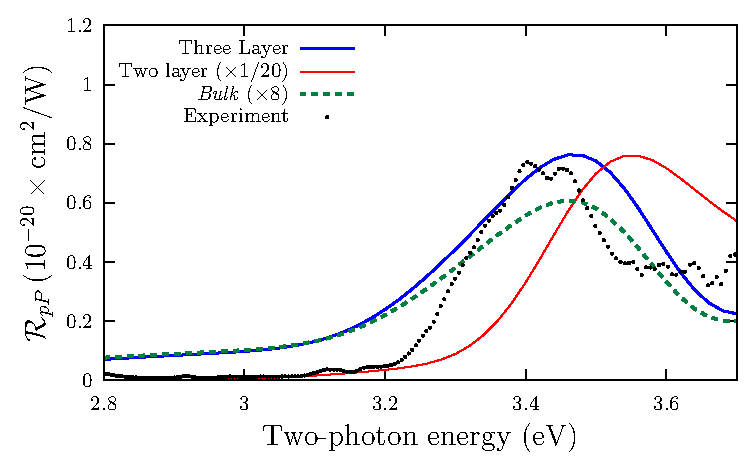
\includegraphics[width=0.48\textwidth]{figures/03-results/shgyield/fig8}
\caption{(Color online) Comparison between theoretical models (see Table
\ref{tab:models}) and experiment for $\mathcal{R}_{pP}$, for
$\theta=45^{\circ}$. We use a scissors value of $\hbar\Delta = 0.7\,\text{eV}$.
The $\chi^{\mathrm{abc}}(-2\omega;\omega,\omega)$ components are broadened with
$\sigma=0.05\,\text{eV}$, and then $\mathcal{R}_{pP}$ is broadened with
$\sigma=0.10\,\text{eV}$. Experimental data taken from Ref.
\cite{mitchellSS01}.\label{fig:mitchellRpP}}
\end{figure}

